% ICRA 2027 submission wrapper — ANONYMIZED for double-anonymous review.
% The paper content lives in body_icra.tex, a page-budget-driven FORK of
% body.tex (shared by mp_main.tex, the T-RO submission).
% body_icra.tex carries the same correctness fixes as body.tex plus
% ICRA-only space cuts (AV steering section, velocity-law table, MPPI/GPU
% related-work prose, and the LQR background subsection compressed or
% dropped) needed to fit the 8-page limit.
% Content edits belonging in every version (correctness/results fixes)
% should still be made in body.tex and re-applied here; edits that are
% purely about saving space belong only in body_icra.tex.
% references_icra.tex is a fork of references.tex dropping two entries
% (apollo, storm2022) that the ICRA-only cuts left uncited; correctness
% fixes to shared entries (e.g. author/title corrections) should still be
% made in references.tex and re-applied here.
% Build: latexmk -pdf mp_main_ICRA.tex
% ICRA 2027 hard limit: 8 pages including references (PaperPlaza, deadline
% 2026-09-15 11:59 PT).
\documentclass[conference]{IEEEtran}
\IEEEoverridecommandlockouts

\usepackage[T1]{fontenc}
\usepackage[utf8]{inputenc}
\usepackage{amsmath,amssymb,amsfonts}
\usepackage{graphicx}
\usepackage{booktabs}
\usepackage{array}
\usepackage{longtable}
\usepackage{calc}
\usepackage{xcolor}
\usepackage{url}
\usepackage{cite}
\usepackage{tikz}
\usetikzlibrary{arrows.meta,positioning,calc,fit,backgrounds}

\graphicspath{{../}}

% ---- shared tikz styles for the architecture schematic ----
\tikzset{
  blk/.style={draw,rounded corners=2pt,align=center,font=\footnotesize,
              minimum height=8mm,inner sep=3pt,fill=blue!4},
  det/.style={draw,rounded corners=2pt,align=center,font=\footnotesize,
              minimum height=8mm,inner sep=3pt,fill=orange!10},
  offb/.style={draw,dashed,rounded corners=2pt,align=center,font=\footnotesize,
              minimum height=8mm,inner sep=3pt,fill=green!6},
  sig/.style={-{Latex[length=2mm]},line width=0.6pt},
  dot/.style={circle,fill,inner sep=1.1pt}
}

% shrink a display equation to the column width only if it would otherwise overflow
\newcommand{\eqfit}[1]{\resizebox{\ifdim\width>\columnwidth \columnwidth\else \width\fi}{!}{\ensuremath{\displaystyle #1}}}

\providecommand{\texorpdfstring}[2]{#1}
\DeclareUnicodeCharacter{2248}{\ensuremath{\approx}}
\DeclareUnicodeCharacter{2022}{\textbullet}

\newcounter{none}
\providecommand{\tightlist}{%
  \setlength{\itemsep}{0pt}\setlength{\parskip}{0pt}}

\makeatletter
\newsavebox\pandoc@box
\newcommand*\pandocbounded[1]{%
  \sbox\pandoc@box{#1}%
  \Gscale@div\@tempa{\textheight}{\dimexpr\ht\pandoc@box+\dp\pandoc@box\relax}%
  \Gscale@div\@tempb{\linewidth}{\wd\pandoc@box}%
  \ifdim\@tempb\p@<\@tempa\p@\let\@tempa\@tempb\fi%
  \ifdim\@tempa\p@<\p@\scalebox{\@tempa}{\usebox\pandoc@box}%
  \else\usebox{\pandoc@box}%
  \fi%
}
\def\fps@figure{tbp}
\makeatother

\setlength{\emergencystretch}{3em}

\begin{document}

\title{Reactive Time-Domain Motion Planning via a Configuration-Independent Double-Integrator Backbone}

% Double-anonymous review: author information omitted (ICRA 2027 rules).
\author{Anonymous~Authors%
\thanks{Manuscript submitted to IEEE ICRA 2027. Author information omitted for double-anonymous review.}%
}

\maketitle
% PaperPlaza compliance: no page numbers (header digits trip the
% margin-imposition check; the submission system adds its own numbering).
\thispagestyle{empty}
\pagestyle{empty}

\begin{abstract}
Traditional motion-planning pipelines separate geometric path generation from time parameterization, making reactive
updates costly when obstacles or task objectives change. This paper presents a unified local Predictive Motion Planner
formulated directly in the time domain. The key observation is architectural: by planning on a virtual double-integrator
backbone rather than on a plant linearization, the state-transition matrix $A_d$ stays constant across configurations,
where a configuration-dependent MPC would have to rebuild its prediction matrices at every cycle. All prediction matrices
can therefore be precomputed offline, and online planning reduces to a convex Quadratic Program (QP) with fixed dynamics
structure.

Within this fixed structure the planner obtains, at the cost of one convex QP per cycle, a combination that path-first pipelines reach only in separate stages: velocity and acceleration limits held exactly by construction, together with reactive replanning that never halts to rebuild a path. The price is global time optimality---a time-optimal parameterization stays 3--3.5$\times$ faster on static paths, quantified in Tables~I--II. The planner optimizes time-indexed joint trajectories on a fixed grid, produces position/velocity profiles $(q_d,\dot q_d)$ with hard-bounded piecewise-constant acceleration $\ddot q_d$, and admits a piecewise-jerk triple-integrator extension when continuous acceleration is required; the same extension carries the principle to autonomous-vehicle lateral planning, where bounding lateral jerk yields a smooth, actuator-rate-feasible steering profile. Benchmarks on a 7-DOF FR3 confirm bounded-latency reactive replanning without the stop-and-rebuild of path-first pipelines. In the single-thread Python harness the decoupled box-constrained QP solves well within the 100 Hz budget and the coupled obstacle QP meets it at p95 with fixed-sparsity updates; rare worst-case cycles exceed 10 ms and would need a compiled solver to remove the tail; the reported timings are diagnostic.
\end{abstract}

\begin{IEEEkeywords}
Motion planning, model predictive control, reactive replanning, real-time trajectory generation, double integrator,
obstacle avoidance, time parameterization.
\end{IEEEkeywords}

\section{Introduction}\label{i.-introduction}

Modern robotic systems deployed in unstructured or human-shared
environments must track planned trajectories with high precision while
remaining responsive to dynamic workspace changes. Classical motion
planning pipelines often address these demands sequentially. A geometric
planner, such as OMPL \cite{ompl}, first searches for a collision-free
path in configuration space. A separate time-parameterization stage, such
as Time-Optimal Trajectory Generation (TOTG) \cite{pham2015},
then maps this spatial path into a timed trajectory through an
arc-length-to-time transformation \(s\rightarrow t\). This separation is
effective for static scenes, but it creates a structural latency issue in
reactive settings: when obstacles or task objectives change, the system
must update the geometric path, the time law, or both before a new
command can be executed. Even when incremental replanners reduce this
latency, the planning stack remains organized around a batch
path-then-time interface rather than a fixed-rate trajectory update.

This paper asks whether the timed trajectory can instead be generated
directly, at the planning rate, while preserving convex kinematic
constraints. The answer rests on an architectural choice rather than a
property of the double integrator itself: an isolated double integrator
is of course linear time-invariant, but a model predictive planner built
on the \emph{physical} plant must re-linearize and rebuild its prediction
matrices at every operating point. By planning instead on a virtual
double-integrator backbone, the state-transition matrix \(A_d\) is held
constant across all robot configurations, so the horizon prediction
matrices can be computed once offline and reused at every replanning
cycle. The online problem is reduced to a convex Quadratic Program (QP)
with fixed dynamics structure; only the current state, reference terms,
and active constraint rows change. The contribution is thus the
substitution of the geometric \(s\rightarrow t\) interface by a
fixed-structure time-domain QP, not the observation that a double
integrator is linear.

The idea is inspired by a two-layer predictive impedance-control
architecture for pHRI \cite{phri}, where dynamic cancellation exposes a
constant double-integrator residual. Here the double integrator is a
\emph{planning backbone}, not a claim about the physical plant: the
planner optimizes reference trajectories for a downstream controller
(computed-torque, impedance, admittance, or other), so the contribution
is a configuration-independent time-domain parameterization enabling
fast repeated QP updates, not a new robot dynamics model.

The resulting framework should be understood as a \textbf{local
predictive motion planner} rather than a complete global planner; we
refer to it throughout as the \textbf{DI-QP planner} (the double-integrator
backbone solved as a receding-horizon QP), and use ``time-first'' only
when contrasting its time-domain structure with the ``path-first'' TOTG
pipeline. It does not perform global search; obstacle avoidance is
handled by linearized safe-corridor rows or by artificial-potential-field
reference deflection, both of which are local mechanisms. Within that scope, 
the framework provides a fixed prediction structure
whose size is independent of robot configuration (growing only with
horizon, dimension, and active rows); direct optimization of time-indexed
joint positions, velocities, and accelerations on a fixed grid; enforcement
of velocity, acceleration, and linearized obstacle constraints inside one
QP; elimination of the separate spatial-to-temporal stage; and continuous
\(C^1\) output with hard-bounded piecewise-constant acceleration, plus a
piecewise-jerk extension when continuous acceleration is required.


\section{Framework and System
Structure}\label{ii.-mathematical-framework-and-system-structure}

\begin{figure*}[t]
\centering
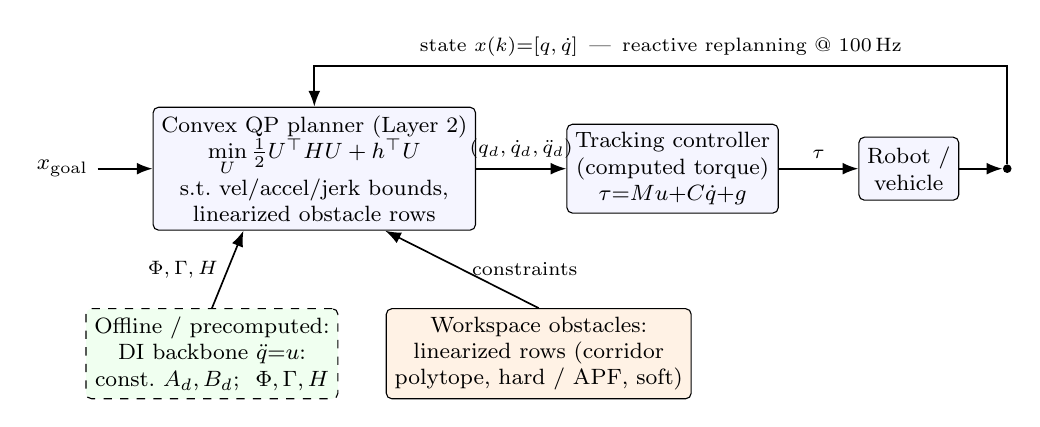
\begin{tikzpicture}[every node/.style={font=\footnotesize}]
  % ---- main execution row ----
  \node (goal) at (0,0) {$x_\text{goal}$};
  \node[blk] (qp) at (3.2,0) {Convex QP planner (Layer~2)\\ $\min\limits_{U}\frac12 U^\top H U+h^\top U$\\ s.t.\ vel/accel/jerk bounds,\\ linearized obstacle rows};
  \node[blk] (ctrl) at (7.75,0) {Tracking controller\\ (computed torque)\\ $\tau{=}Mu{+}C\dot q{+}g$};
  \node[blk] (plant) at (10.75,0) {Robot /\\ vehicle};
  \node[dot] (fb) at (12.0,0) {};
  % forward wires
  \draw[sig] (goal)--(qp);
  \draw[sig] (qp)-- node[above,font=\scriptsize]{$(q_d,\dot q_d,\ddot q_d)$} (ctrl);
  \draw[sig] (ctrl)-- node[above,font=\scriptsize]{$\tau$} (plant);
  \draw[sig] (plant)--(fb);
  % state feedback (reactive replanning)
  \draw[sig] (fb) |- ++(0,1.3) -| node[near start,above,font=\scriptsize]{state $x(k){=}[q,\dot q]$ \,---\, reactive replanning @ 100\,Hz} (qp.north);
  % ---- offline-precompute feeder ----
  \node[offb] (off) at (1.9,-2.35) {Offline / precomputed:\\ DI backbone $\ddot q{=}u$:\\ const.\ $A_d,B_d$;\ \ $\Phi,\Gamma,H$};
  \draw[sig] (off.north) -- node[left,font=\scriptsize,pos=0.5]{$\Phi,\Gamma,H$} ([xshift=-9mm]qp.south);
  % ---- obstacle / perception feeder ----
  \node[det] (obs) at (6.05,-2.35) {Workspace obstacles:\\ linearized rows (corridor\\ polytope, hard / APF, soft)};
  \draw[sig] (obs.north) -- node[right,font=\scriptsize,pos=0.5]{constraints} ([xshift=9mm]qp.south);
\end{tikzpicture}
\caption{Reactive predictive motion-planning architecture. The planner runs on
a virtual \emph{double-integrator backbone} ($\ddot q=u$), whose nilpotent
dynamics give a configuration-independent constant $A_d$, so the horizon
prediction matrices $\Phi,\Gamma$ and the QP Hessian $H$ are precomputed
\emph{offline} (left, dashed). Online, a convex QP (Layer~2) optimizes the
acceleration profile $U$ subject to velocity/acceleration/jerk bounds and
linearized workspace-obstacle rows (convex corridor polytope, hard; or APF goal
deflection, soft), emitting a time-indexed trajectory $(q_d,\dot q_d,\ddot q_d)$
to a downstream tracking controller and plant. Current state $x(k)$ and updated
obstacles re-enter every cycle, giving bounded-latency reactive replanning at
100\,Hz without the stop-and-rebuild of path-first pipelines.}
\label{fig:arch}
\end{figure*}

Let \(q\in\mathbb{R}^n\) denote robot configuration and
\(p=f(q)\) task position. The planner generates
\((q(t),\dot q(t),\ddot q(t))\) satisfying waypoint, joint, velocity,
acceleration, and obstacle constraints; actuator commands are left to a
downstream tracking controller. The trajectory space is parameterized by
a virtual double-integrator backbone,
\begin{equation}
\label{eq:di-backbone}
  \ddot q = u,\qquad
  x=\begin{bmatrix}q^\top&\dot q^\top\end{bmatrix}^\top ,
\end{equation}
whose state contains planned positions and velocities. This model is not
claimed to be the physical plant. It is a configuration-independent
trajectory generator that makes acceleration a decision variable and
therefore keeps velocity and acceleration bounds linear.

\subsection{Double-Integrator Backbone from Dynamic
Cancellation}\label{a.-double-integrator-backbone-from-dynamic-cancellation}

The same backbone can also be derived from the standard manipulator
dynamics \(M(q)\ddot q+C(q,\dot q)\dot q+g(q)=\tau\). With the
computed-torque (inverse-dynamics) feedforward law---the same
cancellation used in the pHRI architecture of \cite{phri}---
\begin{equation}
\label{eq:computed-torque}
  \tau = M(q)u + C(q,\dot q)\dot q + g(q),
\end{equation}
substitution gives the backbone in \eqref{eq:di-backbone}, and hence
\begin{equation}
\label{eq:residual-dynamics}
\dot x = \begin{bmatrix} 0&I\\ 0&0 \end{bmatrix}x +
\begin{bmatrix} 0\\ I \end{bmatrix}u .
\end{equation}
The present work uses this residual model as a planning backbone rather
than as an impedance-regulation controller.

\subsection{Exact ZOH Discretization and the Constant A\_d Property}\label{b.-exact-zoh-discretization-and-the-constant-a_d-property}

Because the continuous system matrix is nilpotent, \(A_c^2=0\), exact
ZOH discretization over \(\Delta t\) gives
\begin{equation}
\label{eq:zoh}
A_d = \begin{bmatrix} 1 & \Delta t \\ 0 & 1 \end{bmatrix}, \qquad
B_d = \begin{bmatrix} \frac{\Delta t^2}{2} \\ \Delta t \end{bmatrix}.
\end{equation}
Unlike a physical plant linearization, this \(A_d\) is independent of
configuration, operating point, and joint index. Therefore the horizon
prediction matrices
\begin{equation}
\label{eq:prediction-matrices}
\Phi = \begin{bmatrix} A_d \\ A_d^2 \\ \vdots \\ A_d^N \end{bmatrix}, \qquad
\Gamma = \begin{bmatrix}
B_d & 0 & \cdots & 0 \\
A_d B_d & B_d & \cdots & 0 \\
\vdots & & \ddots & \vdots \\
A_d^{N-1} B_d & \cdots & A_d B_d & B_d
\end{bmatrix}
\end{equation}
are precomputed once and reused at every planning cycle. Online rollout
then reduces to
\begin{equation}
\label{eq:rollout}
X=\Phi x(k)+\Gamma U,
\end{equation}
decoupling prediction cost from robot configuration.

\section{Receding-Horizon Optimization}\label{iii.-receding-horizon-optimization-layer-2-qp-planner}

\subsection{Optimization Problem
Structure}\label{a.-optimization-problem-structure}

At each planning time step, the planner solves for the optimal
acceleration profile sequence across the prediction horizon:
\begin{equation}
\label{eq:decision-vector}
U = \begin{bmatrix} u^\top(0) & u^\top(1) & \cdots & u^\top(N-1) \end{bmatrix}^\top
\in \mathbb{R}^{nN}.
\end{equation}
where \(n\) is the number of joints and \(N\) is the horizon length
(e.g., \(nN = 7\times 20 = 140\) decision variables for the 7-DOF FR3
with \(N=20\)). The predicted trajectory follows \eqref{eq:rollout},
which is affine in \(U\); therefore kinematic bounds and linearized
obstacle rows remain convex. Absent obstacle coupling, the Hessian is
block-diagonal and the problem separates into \(n\) independent
per-joint QPs of size \(N\).

\subsection{Cost Function: Tracking and
Smoothness}\label{b.-cost-function-tracking-and-smoothness}

The objective function minimizes the weighted sum of tracking deviations
from a goal state \(x_{\text{goal}} = [q_{\text{goal}}, 0]^\top\) and
control effort. We write the stage cost with the conventional
\(\tfrac{1}{2}\) scaling,
\begin{align}
\label{eq:tracking-cost}
J(U)
&=\frac{1}{2}
\left(\Phi x(k)+\Gamma U-\mathbf{1}_N\otimes x_{\text{goal}}\right)^\top
\bar Q \nonumber\\
&\quad \times
\left(\Phi x(k)+\Gamma U-\mathbf{1}_N\otimes x_{\text{goal}}\right)
+\frac{1}{2}U^\top\bar R U .
\end{align}
so that collecting the terms depending on \(U\) gives
\begin{equation}
\label{eq:qp-objective}
\min_{U} \; \frac{1}{2} U^\top H U + h^\top U
\end{equation}
where:
\begin{equation}
\label{eq:qp-hessian-gradient}
H = \Gamma^\top \bar{Q} \Gamma + \bar{R}, \qquad
h = \Gamma^\top \bar{Q} \, x_{\text{free,err}}
\end{equation}
and
\(x_{\text{free,err}} = \Phi x(k) - \mathbf{1}_N \otimes x_{\text{goal}}\)
is the unforced deviation from the goal; \(h\) is the gradient at \(U=0\),
i.e.\ the linear-cost vector passed to OSQP. The remaining definitions
are: the full goal state \(x_{\text{goal}}=[q_{\text{goal}},0]^\top\)
replicated across all \(N\) horizon steps; stage weights
\(Q = \text{blkdiag}(K_q, D_q)\) on position/velocity error; control cost
\(R\) regularizing acceleration; terminal weight \(Q_f = \gamma Q\)
(\(\gamma \approx 5\)--\(10\)); and horizon-stacked
\(\bar Q = \mathrm{blkdiag}(Q,\dots,Q,Q_f)\), \(\bar R = I_N \otimes R\).

Because \(H\) is the sum of a positive semi-definite matrix (from
\(\bar{Q}\)) and a positive definite matrix (from \(\bar{R}\) with
\(R \succ 0\)), the QP is \textbf{strictly convex} for all
configurations and all time steps. A unique global minimizer exists and
is found efficiently by operator-splitting solvers such as OSQP \cite{osqp}
with warm-starting, converging in under 0.5 ms for the decoupled
box-constrained QP and in a few milliseconds for the coupled-obstacle QP
(Section~\ref{b.-fr3-manipulator-results}).

\textbf{Weight tuning guidance.} \(K_q\) sets convergence aggressiveness,
\(D_q\!\approx\!2\sqrt{K_q}\) gives critical damping, \(R\) trades
smoothness against speed, and \(\gamma=5\)--\(10\) compensates the finite
horizon at \(N\geq20\). The FR3 experiments use \(K_q=100\), \(D_q=20\),
\(R=0.1\,I\), \(\gamma=8\) (per-joint scalar), tuned by increasing
\(K_q\) until goals are reached within limits, then \(D_q\) for overshoot,
then \(R\) for excess jerk.

\subsection{Kinematic Hard
Constraints}\label{c.-kinematic-hard-constraints}

Physical joint limits are enforced as hard inequality constraints on the
predicted state and input sequences. For each joint \(i\) and each step
\(k\) along the horizon:
\begin{align}
\label{eq:kinematic-bounds}
-\dot{q}_{i,\max} &\leq \dot{q}_{i}(k) \leq \dot{q}_{i,\max},
&& k=1,\dots,N, \nonumber\\
-u_{i,\max} &\leq u_i(k) \leq u_{i,\max},
&& k=0,\dots,N-1 .
\end{align}

Since the predicted states are affine in \(U\) by \eqref{eq:rollout},
the bounds in \eqref{eq:kinematic-bounds} translate to linear inequalities
\(C_{\text{kin}} U \leq d_{\text{kin}}\) assembled once from the
precomputed \(\Gamma\) matrix and fixed online. Optionally, joint
position limits \(q_{i,\min} \leq q_i(k) \leq q_{i,\max}\) can be
appended with no additional computational overhead.

Because the velocity bounds are imposed without slack, feasibility of the
QP assumes the current state lies inside the velocity polytope; if a
disturbance drives \(\dot q(k)\) outside it, the box rows should be
softened on the first horizon step or a terminal maximal-braking-to-rest
set appended to recover recursive feasibility (see
Section~\ref{scope-and-limitations}).

\section{Incorporating Workspace Obstacle
Avoidance}\label{iv.-incorporating-workspace-obstacle-avoidance}

The linearity of the predicted joint positions with respect to \(U\)
makes it straightforward to incorporate obstacle avoidance constraints
without breaking convexity. Two complementary methods are presented.

\subsection{Convex Corridor Polytope Constraints (Hard
Constraints)}\label{a.-convex-corridor-polytope-constraints-hard-constraints}

Cartesian obstacles detected by perception systems are represented as
half-space inequalities in task space:
\begin{equation}
\label{eq:workspace-halfspace}
A_{\text{obs}} \, p(k) \leq b_{\text{obs}}
\end{equation}
where \(p(k) \in \mathbb{R}^3\) is the predicted end-effector (or link)
position at step \(k\). Using the robot's forward kinematics linearized
at the current operating point via the translational Jacobian
\(J_v(q_0)\):
\begin{equation}
\label{eq:fk-linearization}
p(k) \approx p_0 + J_v(q_0)\bigl(q(k) - q_0\bigr)
\end{equation}
the workspace constraint in \eqref{eq:workspace-halfspace} becomes:
\begin{equation}
\label{eq:workspace-linear-row}
A_{\text{obs}} J_v(q_0) \, \Delta q(k)
\leq b_{\text{obs}} - A_{\text{obs}} p_0
\end{equation}
where \(\Delta q(k) = q(k) - q_0\) is linear in \(U\) through
\(\Gamma\). To make the QP row explicit, let
\(E_{q,k}\in\mathbb{R}^{n\times 2nN}\) be the selector that extracts the
\(n\)-dimensional joint-position block of the stacked state \(X\) at
horizon step \(k\) (a row of \(n\times n\) identity blocks, zero
elsewhere), so
\begin{equation}
\label{eq:position-selector}
q(k)=E_{q,k}\bigl(\Phi x(k_0)+\Gamma U\bigr).
\end{equation}
Define \(C_{\text{obs},k}=A_{\text{obs}}J_v(q_0)E_{q,k}\Gamma\). Then
each obstacle row has the affine form
\begin{equation}
\label{eq:obstacle-row}
\begin{aligned}
 C_{\text{obs},k}U
&\le b_{\text{obs}}-A_{\text{obs}}p_0 \\
&\quad
-A_{\text{obs}}J_v(q_0)\bigl(E_{q,k}\Phi x(k_0)-q_0\bigr)
=: d_{\text{obs},k}.
\end{aligned}
\end{equation}
Thus the free-response term is absorbed into the right-hand side, and
the obstacle constraint becomes a set of affine inequalities in \(U\),
fully compatible with the convex QP structure.

\textbf{Approximation quality.} Because \(J_v(q_0)\) is held constant over
the horizon, these rows are a first-order local approximation---exact near
\(q_0\), increasingly inaccurate away from it. Re-linearizing every cycle
refreshes it; a conservative half-space additionally tightens each row by
a bound on the linearization error. From the second-order Taylor
remainder, with \(H_p(q_0)\) the position Hessian,
\begin{equation}
\label{eq:linearization-error}
\|p(q) - (p_0 + J_v(q_0)\Delta q)\|
\leq \tfrac{1}{2} \|H_p(q_0)\|_F \|\Delta q\|^2,
\end{equation}
so an obstacle row \(a^\top p\le b\) tightens to
\(a^\top(p_0+J_v(q_0)\Delta q(k))\le b-\|a\|\,\varepsilon_p\) with
\(\varepsilon_p\) set from \eqref{eq:linearization-error}. For the FR3,
\(\|H_p\|_F\) sampled at 5000 configurations has mean \(1.64\),
95th-percentile \(1.96\)\,m/rad\(^2\), and the measured end-horizon error
grows quadratically with joint-speed\(\times\)horizon (7.1\,mm at 25\%
speed over 0.1\,s, 106.4\,mm at 50\% over 0.2\,s, 1.03\,m at full speed
over 0.4\,s)---well below the Frobenius bound's worst case
(\(\approx\)1.0\,m at 50\% speed), since the executed motion does not
excite the worst-case curvature. In practice the margin should be set
from the \emph{measured} drift rather than the conservative Frobenius
bound, with the horizon shortened for fast motions; at modest speeds a
centimetre-scale margin suffices.

\textbf{Accuracy of the constraint guarantee.} The QP guarantees
satisfaction of the \emph{linearized} safe-corridor constraints: no
predicted trajectory penetrates the declared linearized obstacle polytope.
A true nonlinear collision-clearance guarantee additionally requires
conservative tightening by \(\varepsilon_p\), nonlinear collision checking
of the accepted rollout, or both; for non-convex environments, standard
safe-corridor decomposition \cite{safe_corridor} can be applied upstream.

\textbf{Multiple obstacles.} Method A appends \(M\) independent half-space
sets, keeping convexity at mildly increasing solver cost; if rows conflict
the QP becomes infeasible, resolved by per-obstacle slacks \(s_m \geq 0\)
with penalty \(\mu \|s\|^2\). Method B sums individual APF repulsion
fields, avoiding infeasibility but inheriting the local-minimum risk of
scalar APF methods.

\subsection{Artificial Potential Field Target Deflection (Soft
Constraint)}\label{b.-artificial-potential-field-target-deflection-soft-constraint}

For scenarios requiring maximum solver throughput, an alternative
soft-constraint approach using Artificial Potential Fields (APF) \cite{khatib1986}
is available. An obstacle at position \(p_{\text{obs}}\) with influence
radius \(\rho_0\) and repulsive gain \(\eta\) generates a task-space
repulsive potential:
\begin{equation}
\label{eq:apf-potential}
\mathcal{U}_{\text{rep}}(p) =
\begin{cases}
\frac{1}{2} \eta
\left(\frac{1}{\|p - p_{\text{obs}}\|} - \frac{1}{\rho_0}\right)^2,
& \|p - p_{\text{obs}}\| \leq \rho_0,\\
0, & \text{otherwise}.
\end{cases}
\end{equation}
The negative gradient
\(g_{\text{rep}}(p)=-\nabla \mathcal{U}_{\text{rep}}(p)\), treated as a
synthetic direction field rather than a physical force, is normalized as
\(\hat{g}_{\text{rep}}=g_{\text{rep}}/(\|g_{\text{rep}}\|+\epsilon)\) and
mapped to a heuristic joint-space target shift via the Jacobian
pseudo-inverse,
\begin{equation}
\label{eq:apf-target-shift}
\delta q_{\text{obs}} = K \, J_v^+(q) \, \hat{g}_{\text{rep}},
\end{equation}
where the scalar gain \(K > 0\) absorbs all dimensional scaling. (In the
simulations below the same idea is implemented as a velocity/reference
deflection with an optional tangential component to avoid stalls; in both
cases APF changes the reference rather than adding a hard row.) The target
fed to the cost function is then updated online:
\begin{equation}
\label{eq:apf-target}
q_{\text{target}}(k) = q_{\text{goal}} + \delta q_{\text{obs}} .
\end{equation}
This bypasses inequality rows entirely, preserving the minimal QP
structure and maximizing solve speed. The trade-off is that obstacle
avoidance is enforced softly through the cost function rather than
guaranteed through hard constraints; APF-based avoidance is also
susceptible to local minima in complex environments (see Section VIII).

\textbf{Local minima mitigation.} When the APF gradient vanishes the
planner stalls; three escape strategies are available---waypoint
injection after a no-progress timeout, a small random perturbation to
\(q_\text{target}\), or a hybrid switch to the Method-A hard polytope
(with slack) on stall---of which waypoint injection is preferred since it
adds no solver overhead. The two methods are complementary: hard polytope
constraints for static infrastructure, APF deflection for dynamic
obstacles.

\section{Architectural Properties}\label{v.-architectural-properties}

\subsection{Constant-Structure MPC, Bounded Latency, and
\texorpdfstring{\(C^1\)}{C1}
Output}\label{a.-constant-structure-mpc-and-bounded-replanning-latency}

All dynamics prediction matrices (\(\Phi\), \(\Gamma\), \(H\)) are
precomputed offline and never rebuilt online; obstacle rows are
re-assembled each cycle but still project \(J_v\) through the fixed
\(\Gamma\). Each cycle thus executes a QP whose dynamics structure is
fixed at initialization, so replanning latency is bounded by one QP solve
for a given active set---growing with the obstacle-row count but
independent of configuration and free of prediction-matrix rebuilds. This
is distinct from configuration-dependent MPC (which recomputes prediction
matrices at each linearization point) and from batch planning (TOTG,
TOPP-RA, where any workspace change triggers a full rebuild); the
constant-\(A_d\) property is what makes bounded per-cycle reactivity
achievable in a convex formulation. Because the framework has no
geometric path---positions, velocities, and accelerations along the
horizon are generated simultaneously in one QP---the \(s\leftrightarrow
t\) conversion stage and its singularities (Section VI-A) are eliminated
by construction. And because joint acceleration \(u_i\) is the direct
optimization variable under hard bounds, the output \((q_d,\dot q_d)\) is
\(C^1\) with \(\ddot q_d\) hard-bounded and piecewise-constant (held over
each zero-order-hold control cycle); full \(C^2\) continuity requires
jerk as the optimization variable, as in the extension below.

\subsection{Piecewise-Jerk Triple-Integrator Extension}\label{d.-piecewise-jerk-triple-integrator-extension-for-continuous-acceleration}

When continuous acceleration is required---to reduce torque-rate
excitation, satisfy comfort limits, or bound steering-rate in vehicle
applications---the same constant-\(A_d\) principle extends to a
triple-integrator backbone that optimizes jerk \(\dddot q_i = j_i\) on the
state \(z_i=[q_i,\dot q_i,\ddot q_i]^\top\). The continuous system matrix
is again nilpotent (\(A_c^3=0\)), so exact ZOH discretization gives the
configuration-independent
\begin{equation}
\label{eq:triple-zoh}
A_d^{(3)} =
\begin{bmatrix}
1&\Delta t&\tfrac{1}{2}\Delta t^2\\
0&1&\Delta t\\
0&0&1
\end{bmatrix},
\qquad
B_d^{(3)} =
\begin{bmatrix}
\tfrac{1}{6}\Delta t^3\\
\tfrac{1}{2}\Delta t^2\\
\Delta t
\end{bmatrix}.
\end{equation}
so the prediction matrices remain precomputable offline. With jerk held
constant per interval, \(\ddot q(t+\tau)=\ddot q(t)+\tau j(t)\) keeps
acceleration continuous across samples while jerk is piecewise-constant,
raising output smoothness from \(C^1\) to \(C^2\) (\(q_d\in C^2\),
\(\dot q_d\in C^1\), \(\ddot q_d\in C^0\)) with hard linear bounds now
available on velocity, acceleration, and jerk.

The trade-off is a larger state and extra predicted-state rows, though the
decision sequence is still length \(nN\), now a jerk sequence
\(J=[j(0),\dots,j(N-1)]\) rather than acceleration. The AV steering-rate
benchmark (§VI.C) uses exactly this for the lateral channel, since steering
rate depends on lateral jerk.

The rest of the paper uses the double-integrator backbone as the main
manipulator planner because it is the smallest model that enforces
velocity and acceleration limits directly and gives the fastest QP. The
triple-integrator form is a drop-in extension when continuous
acceleration or explicit jerk bounds are application-critical.

The unconstrained infinite-horizon limit of the planner is the standard LQR
law \(u=u_{ff}-K(x-x_r)\), situating the constrained, finite-horizon planner
as its receding-horizon QP counterpart---mathematically close to linear MPC
\cite{mayne2000}, but on a virtual trajectory state rather than a plant
linearization; the robot model enters only through kinematics and workspace
constraints \cite{khatib1987}, and the output is the reference trajectory
\(\mathcal T=\{q_d,\dot q_d,\ddot q_d\}\) for a downstream controller.

\section{Experimental Evaluation}\label{vi.-experimental-evaluation}

We evaluate the proposed planner against a path-first Time-Optimal
Trajectory Generation pipeline on a 7-DOF Franka FR3 manipulator and on
an autonomous-vehicle steering task. Both planners receive identical
waypoints and kinematic limits and emit \((q_d, \dot q_d, \ddot q_d)\)
sampled at the same \(\Delta t\); all numbers reported below are
measured by the accompanying open harness (\texttt{simulationResults/}). The
TOTG reference uses the numerical-integration TOPP core---circular-blend
path (Kunz--Stilman geometry \cite{kunz2012}), time-optimal forward/backward
sweep on \(\dot s^2\) \cite{toppra}, then \(s\!\to\!t\) inversion and
resampling.

\textbf{Scope of comparison.} We compare against the path-first family
(TOTG, TOPP-RA), a resolved-rate-plus-APF baseline, and a sampling-based
MPPI baseline on the planar dynamic-obstacle test
(Section~\ref{d.-bounded-latency-reactive-replanning}). Online nonlinear MPC
and CHOMP/TrajOpt are deferred to future work; the present planner's appeal
is precisely the constant-\(A_d\) precomputation and bounded per-cycle
latency that richer nonlinear formulations forego.

This section reports four evaluation axes: reactive latency, jerk/
smoothness, constraint fidelity, and the execution-time gap. The point is
not that the proposed planner is uniformly faster than time-optimal path
parameterization on static paths; it is not. Rather, the fixed time-domain
QP trades a small amount of global time optimality for bounded reactive
updates, explicit limit satisfaction, and smoother command profiles.

\subsection{\texorpdfstring{Path-First \(t\!\leftrightarrow\!s\)
Conversion Artifacts}{Path-First t-s Conversion Artifacts}}\label{a.-path-first-tleftrightarrows-conversion-artifacts}

The \(s\!\to\!t\) reconstruction differentiates the geometric path,
\[\eqfit{\ddot q(t) = q'(s)\,\ddot s \;+\; \underbrace{q''(s)}_{\text{curvature vector}}\,\dot s^2 .}\]
Two pathologies follow from the standard circular-blend path
representation. First, \(q''(s)\) jumps at every blend seam (\(0\) on a
straight segment, \(1/r\) on a circular arc), so the reconstructed
\(\ddot q\) is discontinuous, with the jump scaling as \(\dot s^2\).
Second, \(t(s)=\int ds/\dot s\) is singular wherever \(\dot s \to 0\)
(rest points, tight near-reversal blends), making the uniform-time
resample ill-conditioned. These artifacts are a property of the
circular-blend path representation, not of time parameterization per se.
Replacing circular blends with a \(C^2\) path (e.g., cubic splines)
removes them, as confirmed below. The time-first planner never forms
\(s\); its \(\ddot q\) is the bounded decision variable, so neither
pathology can arise.

In the \((s,\dot s)\) phase plane (TOPP-RA style), the maximum-velocity
curve and optimal profile \(\dot s^*(s)\) dip toward zero at the tight
blend---severely on the near-reversal, where \(\dot s\to0\) drives
\(t(s)\) singular.

\subsection{FR3 Manipulator
Results}\label{b.-fr3-manipulator-results}

Stresses are concentrated in two joints for interpretability, though all
seven are planned. The decisive metric is the peak acceleration ratio
\(\lVert\ddot q\rVert_\infty/\ddot q_{\max}\): above \(1\) means the
emitted trajectory violates the declared limit. Because the DI planner
enforces this as a hard QP constraint, it is pinned at \(1.000\) with
zero violations \emph{by construction}; the informative comparison is how
far TOTG departs from that bound.

{% converted Pandoc table
\begin{table*}[t]
\caption{FR3 Manipulator Benchmark Results}
\label{tab:fr3-main-results}
\centering
\footnotesize
\setlength{\tabcolsep}{3pt}
\begin{tabular}{@{}
  >{\raggedright\arraybackslash}p{(\linewidth - 14\tabcolsep) * \real{0.1250}}
  >{\raggedright\arraybackslash}p{(\linewidth - 14\tabcolsep) * \real{0.1250}}
  >{\raggedright\arraybackslash}p{(\linewidth - 14\tabcolsep) * \real{0.1250}}
  >{\raggedright\arraybackslash}p{(\linewidth - 14\tabcolsep) * \real{0.1250}}
  >{\raggedright\arraybackslash}p{(\linewidth - 14\tabcolsep) * \real{0.1250}}
  >{\raggedright\arraybackslash}p{(\linewidth - 14\tabcolsep) * \real{0.1250}}
  >{\raggedright\arraybackslash}p{(\linewidth - 14\tabcolsep) * \real{0.1250}}
  >{\raggedright\arraybackslash}p{(\linewidth - 14\tabcolsep) * \real{0.1250}}@{}}
\toprule\noalign{}
\begin{minipage}[b]{\linewidth}\raggedright
Scenario
\end{minipage} & \begin{minipage}[b]{\linewidth}\raggedright
DI \(T\) {[}s{]}
\end{minipage} & \begin{minipage}[b]{\linewidth}\raggedright
TOTG \(T\) {[}s{]}
\end{minipage} & \begin{minipage}[b]{\linewidth}\raggedright
DI accel ratio
\end{minipage} & \begin{minipage}[b]{\linewidth}\raggedright
TOTG accel ratio
\end{minipage} & \begin{minipage}[b]{\linewidth}\raggedright
TOTG accel viol.
\end{minipage} & \begin{minipage}[b]{\linewidth}\raggedright
DI jerk RMS
\end{minipage} & \begin{minipage}[b]{\linewidth}\raggedright
TOTG jerk RMS
\end{minipage} \\
\midrule\noalign{}
B1 point-to-point & 2.02 & \textbf{0.59} & 1.000 & 1.000 & 0 &
\textbf{22} & 143 \\
B2 acute corner (tight blend) & 1.92 & \textbf{1.23} & 1.000 &
\textbf{1.047} & 2 & 36 & 133 \\
B3 near-reversal & 1.99 & 1.07 & 1.000 & up to \textbf{3.13} & 0--1 & 29
& 166 \\
B4 dense (24 waypoints) & 13.24 & \textbf{3.83} & 1.000 & \textbf{1.445}
& 49 & \textbf{54} & 333 \\
\bottomrule\noalign{}
\end{tabular}
\end{table*}
}

Separating the decoupled and coupled cases, the single-threaded Python
harness (OSQP tolerance \(10^{-6}\), warm-started, fixed KKT sparsity on
the coupled update path) solves the 140-variable decoupled box-constrained
QP (7 DOF, \(N{=}20\)) in 0.05--0.09 ms mean ($\sim$0.4 ms worst; 0.03 ms
for a warm-started goal reaction) and the 141-variable coupled obstacle QP
(Method A, fixed-sparsity) in 2.1 ms mean / 9.5 ms worst.

A horizon sweep \(N=\{10,20,30,40\}\) on the same coupled FR3
dynamic-obstacle problem (\texttt{sweep\_N.py}) confirms why \(N=20\)
(0.2 s) is the default. Because the scenario uses a velocity-law/APF
reference, completion (1.83--1.86 s) and min EE clearance ($\approx$0.30 m)
are nearly insensitive to \(N\); the dominant trend is computational, with
coupled-QP solve p95 rising steeply from 1.0 ms (\(N{=}10\)) and 4.4 ms
(\(N{=}20\)) to 20.4 ms (\(N{=}30\)) and 55.6 ms (\(N{=}40\)). For pure
position-tracking waypoints \(N=10\) instead inflates time-to-goal, so
\(N=20\) balances both regimes.

\textbf{Comparison scope.} The acceleration violation metric compares
the trajectory as emitted by each planner---i.e., the command sequence
as-sent to the controller, with no downstream smoothing or
re-interpolation applied to either planner's output. In practice, some
systems apply a final spline pass to the TOTG output before execution,
which would reduce or eliminate the resampling-induced violations on B2
and B4; under such post-processing the DI planner's zero-violation
advantage on those scenarios shrinks. The advantage on B3 (near-reversal
singularity) and in the reactive scenarios (Sections VI.D--E) is
independent of downstream smoothing.

Figure~\ref{fig:fr3-accel-compare} plots the acceleration ratio over time
for each scenario: the DI curve never crosses \(1\), while the TOTG curve
spikes above it at blend seams.

\begin{figure}[t]
\centering
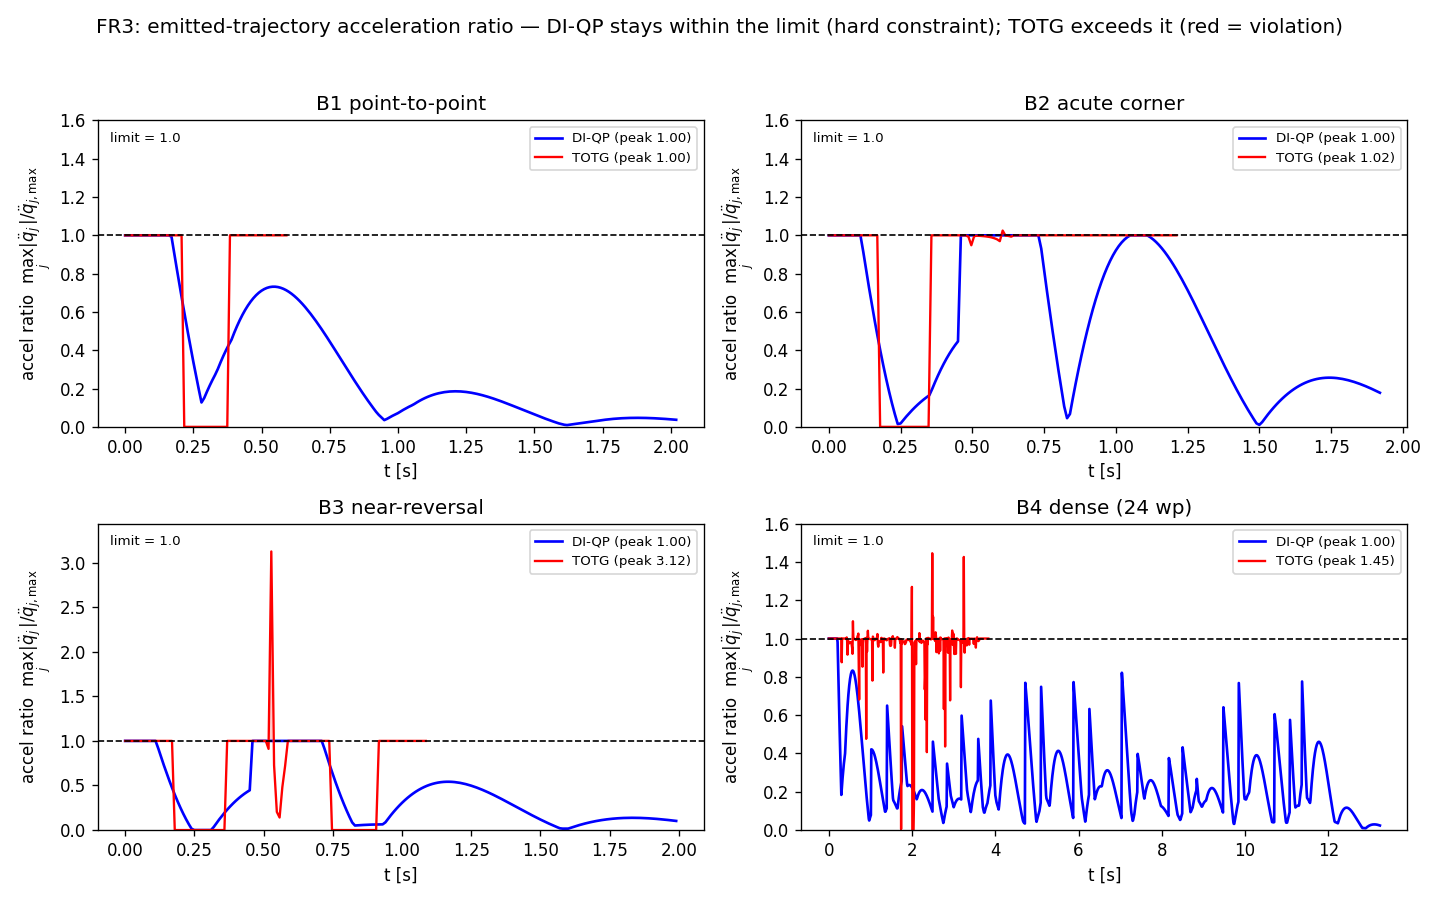
\includegraphics[width=\linewidth]{simulationResults/fr3_accel_compare.png}
\caption{FR3 emitted-trajectory acceleration ratio
\(\max_j|\ddot q_j|/\ddot q_{j,\max}\) over time, DI-QP (blue) vs TOTG
(red), B1--B4; dashed line is the limit. DI-QP is pinned within the limit
by hard constraints; TOTG exceeds it at blend seams (B2 \(1.047\times\),
B3 up to \(3.13\times\), B4 \(1.445\times\)). The B3 spike is
blend-dependent (drops to \(1.00\times\) under TOPP-RA/\(C^2\)); the
intrinsic path-first issues are the \(\dot s\to0\) singularity and
curvature-discontinuous reconstruction, not the spike magnitude.}
\label{fig:fr3-accel-compare}
\end{figure}

In \textbf{B3 (near-reversal)} the blend radius collapses,
\(\dot s\to 0\), and the parameterization becomes singular:
\(\max(1/\dot s)\to\infty\) and the \(s\!\to\!t\) conversion fails
(flagged and capped by the harness). In \textbf{B4} the path-first
command breaks the acceleration limit by 45\% at 49 samples. The DI
planner remains feasible and smooth throughout.

\textbf{Robustness to the parameterizer (TOPP-RA).} Re-running with
reachability-based TOPP-RA \cite{toppra} confirms the findings persist
(acute corner \(1.020\times\), dense path \(1.12\times\), near-reversal
still singular) while softening magnitudes (the B3 spike drops from
\(3.13\times\) to \(1.000\times\)), separating implementation-dependent
spike size from the intrinsic path-first issues (curvature-discontinuous
reconstruction, the \(\dot s\to0\) singularity). Replacing circular
blends with a \(C^2\) spline removes the B2/B4 violations entirely, so
TOPP-RA on a \(C^2\) path is a competitive baseline the DI planner does
not strictly dominate on those metrics.

\textbf{Time-optimality.} TOTG is the lower bound by construction, and
the quadratic-cost DI planner pays for its smoothness in time (B1
\(3.4\times\), B4 \(3.5\times\) slower). Supplying an analytic
time-optimal velocity-law reference (velocity-dominant weights) recovers
the gap to \(1.06\)--\(1.32\times\) while the DI-QP still preserves zero
limit violations, at the cost of raising jerk RMS by roughly an order of
magnitude---the velocity-law reference is thus an explicit
speed-versus-smoothness selector, not a strictly dominant setting. The DI
planner remains feasible by construction with respect to the declared
time-domain bounds, while path-first feasibility can be lost after
circular-blend reconstruction and uniform-time resampling unless a
smoother path representation or downstream post-processing is used.

\subsection{Illustrative Extension: Vehicle Steering-Rate
Smoothness}\label{c.-autonomous-vehicle-motion-planning-with-the-double-integrator-backbone}

The same backbone extends to autonomous-driving stacks that separate a
Cartesian double integrator \(\ddot p=u\) from steering/throttle control,
recovering heading and curvature as
\(\theta=\operatorname{atan2}(\dot y,\dot x)\),
\(\kappa=(\dot x\ddot y-\dot y\ddot x)/(\dot x^2+\dot y^2)^{3/2}\). This is a
preliminary illustration, not a full kinematic-bicycle planner: on a
lane-change maneuver with a representative 0.5\,rad/s steering-rate cap, the
jerk-bounded time-first extension stays within the cap (peak rate
0.130\,rad/s) while the path-first command exceeds it on the double lane
change (0.594\,rad/s) because circular-blend curvature steps at path seams; a
full bicycle-model treatment is left to future work.

\subsection{Bounded-Latency Reactive
Replanning}\label{d.-bounded-latency-reactive-replanning}

The reactivity advantage is structural rather than
implementation-dependent. A planar point robot must reach a goal while a
disk obstacle crosses its straight-line path mid-execution. The DI
planner recomputes an APF velocity reference from the obstacle's current
position each 100 Hz cycle and re-solves the box-constrained QP,
deflecting continuously. The path-first planner must halt, rebuild a
detour path, and re-run TOPP from rest.

Both reach the goal collision-free, but with very different cost
structure. In this fixed-size APF benchmark, the DI planner's
\textbf{worst reaction latency is \(0.70\) ms}: it is one warm-started QP
update rather than a geometric path rebuild, and its completion time
stays flat at \(6.53\)\,s regardless of added path-search latency. TOTG,
which must halt and rebuild, degrades as that latency grows: completion
rises from \(6.28\)\,s (halted \(0.08\)\,s) at zero added latency to
\(7.18\)\,s (halted \(1.26\)\,s) at \(400\)\,ms. The reactive edge is
decisive when replanning is expensive (full geometric search) or
obstacles are fast, and marginal when the rebuild is cheap; with zero
replan latency, TOTG and DI have comparable completion times, so the DI
planner does not demonstrate lower total throughput.

\textbf{Comparison with a sampling-based reactive baseline.} Since TOTG
isolates the reactivity gap against path-first pipelines specifically, we
also compare against a reactive method that, like ours, never halts:
Model-Predictive Path Integral (MPPI) \cite{williams2017} on the same
planar double integrator and moving obstacle (\(K{=}512\) rollouts,
\(H{=}20\), \(\lambda{=}60,\sigma{=}4\)---the tightest-clearance setting
in a temperature sweep; lower \(\lambda\) turns winner-take-all and fails
to reach the goal). Both reach the goal with essentially identical
safety, but the cost structure differs sharply
(Table~\ref{tab:mppi-compare}): MPPI enforces the velocity limit only by
clamping the applied command---on \(166\) cycles---whereas the DI-QP
enforces it as a convex constraint and never clamps, at roughly
\(10\times\) lower mean compute; bounded-latency reactivity alone is thus
not unique to this planner, but pairing it with hard limit feasibility at
QP-level cost is.

{% converted Pandoc table
\begin{table}[t]
\caption{Reactive Baselines on the Planar Dynamic-Obstacle Test}
\label{tab:mppi-compare}
\centering
\footnotesize
\setlength{\tabcolsep}{4pt}
\begin{tabular}{@{}>{\raggedright\arraybackslash}p{0.46\linewidth}rr@{}}
\toprule\noalign{}
Metric & DI-QP & MPPI \\
\midrule\noalign{}
Reached goal & yes & yes \\
Completion time {[}s{]} & 6.53 & 6.12 \\
Min clearance {[}m{]} & 0.485 & 0.483 \\
Velocity limit enforced by & QP constraint & clamping \\
Cycles needing velocity clamp & \textbf{0} & 166 \\
Rollouts per cycle & 1 QP & \(512\times20\) \\
Mean cycle latency {[}ms{]} & \textbf{0.11} & 1.13 \\
Worst cycle latency {[}ms{]} & \textbf{0.70} & 2.2 \\
\bottomrule\noalign{}
\end{tabular}
\end{table}
}

A planar test also exposes the APF method's known failure mode: with a
purely radial field, attractive and repulsive terms balance in front of an
obstacle and the planner stalls (6.07\,m short of the goal). A simple
waypoint-injection rule---detect lack of progress, insert a lateral
detour---recovers the same box-constrained QP to the goal (0.12\,m
residual) at the same clearance and limits, at negligible extra solve
cost; this motivates using hard polytope constraints or explicit waypoint
logic whenever progress stalls or clearance must be certified, with APF
deflection reserved for fast reactive steering.

\subsection{Scaling to the 7-DOF Arm with a Dynamic
Obstacle}\label{f.-scaling-to-the-7-dof-arm-with-a-dynamic-obstacle}

We exercise the full Section IV machinery on the 7-DOF FR3, where obstacle
constraints couple the joints through the translational Jacobian: the arm
reaches a joint-space goal while a spherical obstacle crosses the
end-effector path, compared against a resolved-rate-plus-APF reactive
controller without hard limits. Both avoid the obstacle and reach the
goal, but the reactive baseline exceeds the joint velocity limit at 42
samples and acceleration at 346, whereas the QP holds every joint limit
exactly and keeps the linearized half-space feasible (zero slack), at a
min EE clearance of 0.296\,m versus 0.339\,m for the unconstrained
baseline. The fixed-sparsity coupled-QP solve is 2.1\,ms mean / 4.4\,ms
p95 / 9.5\,ms worst (3.7/5.9/11.1\,ms with Python assembly overhead); the
harness meets 100\,Hz at p95 while worst-case cycles exceed 10\,ms, so a
hard deadline would need a compiled solver with fixed active-set warm
starts, left to implementation work.

\begin{figure}[t]
\centering
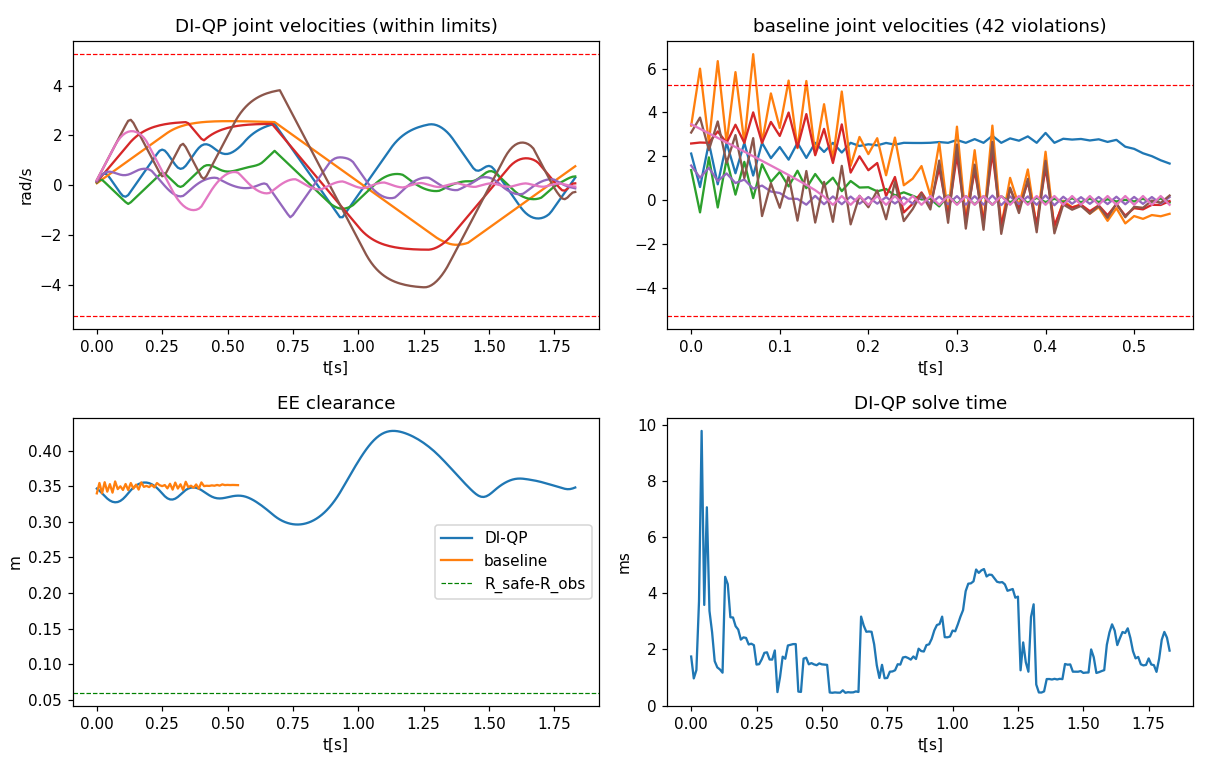
\includegraphics[width=\linewidth]{simulationResults/fr3_dynamic.png}
\caption{7-DOF FR3 dynamic obstacle. Top-left: DI-QP
joint velocities, all within the limit. Top-right: resolved-rate+APF
baseline, which exceeds the velocity limit. Bottom-left: end-effector
clearance. Bottom-right: DI-QP per-cycle solve time.}
\label{fig:fr3-dynamic}
\end{figure}

\subsection{Randomized FR3 Dynamic-Obstacle
Robustness}\label{g.-randomized-fr3-dynamic-obstacle-robustness}

To check that the dynamic-obstacle result is not tied to a single
hand-picked configuration, we perturb the start and goal joint states,
obstacle lateral offset, initial height, and crossing speed over 20
randomized trials (\texttt{fr3\_dynamic\_randomized.py}, seed 7). Both
planners reach the goal in all trials and avoid the obstacle. The
distinction is constraint fidelity: the QP maintains hard joint limits
in every trial, while the resolved-rate baseline repeatedly exceeds
them.

{% converted Pandoc table
\begin{table}[t]
\caption{Randomized FR3 Dynamic-Obstacle Robustness}
\label{tab:fr3-randomized}
\centering
\footnotesize
\setlength{\tabcolsep}{3pt}
\begin{tabular}{@{}>{\raggedright\arraybackslash}p{0.46\linewidth}rr@{}}
\toprule\noalign{}
Metric & DI-QP & Reactive baseline \\
\midrule\noalign{}
Success rate & 100\% & 100\% \\
Min EE clearance, mean ± std {[}m{]} & 0.293 ± 0.018 & 0.328 ± 0.021 \\
Worst min EE clearance {[}m{]} & 0.261 & 0.266 \\
Total joint velocity violations & \textbf{0} & 618 \\
Total joint acceleration violations & \textbf{0} & 6889 \\
Max slack used {[}m{]} & 0.0000 & --- \\
QP solve p95 / max {[}ms{]} & ≈5.2 / ≈15 & --- \\
\bottomrule\noalign{}
\end{tabular}
\end{table}
}

The baseline tends to keep slightly larger clearance because it is
unconstrained and can command arbitrarily aggressive joint velocities
and accelerations. The QP accepts a smaller but still positive clearance
while preserving every declared joint limit.

The three worst-case timings reported in this paper---9.5\,ms bare-solve,
11.1\,ms with Python assembly overhead, and 14--15\,ms over this
randomized tail---measure progressively more of the pipeline; the p95
stays within a few milliseconds in all three, so only the rare tail
cycles, not the median, would need a compiled solver and fixed active-set
warm starts to meet a hard 10\,ms deadline.

\subsection{Physical Execution in
MuJoCo}\label{h.-physical-execution-in-mujoco}

To verify that planner-level differences survive contact with rigid-body
dynamics, we execute both references on a torque-controlled FR3 in
MuJoCo (3.8.1; full mass matrix and gravity). A \(500\) Hz
computed-torque controller tracks each \(100\) Hz reference on the
acute-corner maneuver.

{% converted Pandoc table
\begin{table}[t]
\caption{MuJoCo Computed-Torque Execution}
\label{tab:mujoco-execution}
\centering
\footnotesize
\setlength{\tabcolsep}{3pt}
\begin{tabular}{@{}lcc@{}}
\toprule\noalign{}
Metric (joint 1 / worst) & DI-QP & TOTG \\
\midrule\noalign{}
Peak demanded torque {[}Nm{]} & 58.0 & 56.7 \\
Torque-rate RMS {[}Nm/s{]} & \textbf{181} & 383 \\
Samples over torque limit & 0 & 0 \\
Tracking RMSE {[}mrad{]} & 1.9 & 2.0 \\
\bottomrule\noalign{}
\end{tabular}
\end{table}
}

Both stay within the torque envelope and track to \(\approx\)2\,mrad RMS,
but TOTG's acceleration discontinuity at the blend seam manifests
physically as a stepped torque command (torque-rate RMS \(2.1\times\)
that of the DI reference) and completes the fixed path faster, while the
DI reference is smoother and gentler on the drivetrain---the
smoothness-versus-time trade-off in closed-loop physics rather than at
the planner output.

\section{Implementation Notes}\label{vii.-implementation-notes}

The QP is solved with OSQP \cite{osqp}. \textbf{Warm-starting} from the
previous solution \(U^*\) cuts cold-start latency from $\sim$5\,ms to
under 0.5\,ms for the decoupled box-constrained QPs, and \textbf{sparse
structure} is reused throughout: \(H\) is assembled once offline, and the
coupled-obstacle half-space uses a fixed sparsity pattern updated in
place, avoiding symbolic re-factorization each cycle. \(N=20\) (0.2\,s)
is the default \textbf{horizon length}---\(N=10\) is too short for
position-tracking waypoints, while \(N\approx30\) only narrows the static
time-optimality gap at higher jerk and solve time. For multi-waypoint
tasks the goal is advanced online as waypoints are reached, with no path
splicing or re-initialization; online cost is dominated by the QP solve
itself (\(nN=140\) variables for the 7-DOF \(N{=}20\) case), since the
precomputed \(\Phi,\Gamma\) are never rebuilt---the practical payoff of
the constant-\(A_d\) property.

\section{Discussion}\label{viii.-discussion}

\textbf{Scope and limitations.}\label{scope-and-limitations}
This is a \textbf{local} predictive planner bounded by
four limitations. \textbf{(i) Not time-optimal by default:} a
pure position-tracking cost regulates like a damped second-order system,
inflating time-to-goal to \(3\)--\(3.5\times\) TOTG; the analytic
velocity-law reference recovers this to \(1.06\)--\(1.32\times\) at zero
violations, acting as a speed-versus-smoothness selector. \textbf{(ii)
Linearization accuracy:} Method-A Jacobian linearization is accurate only
locally, with error growing quadratically in joint-speed$\times$horizon
($\approx$10 cm at 50\% speed over 0.2 s), so fast or large-detour motions
need a shorter horizon, an inflated Hessian-bound margin, or nonlinear
rollout checking. \textbf{(iii) Local minima:} Method-B APF can stall;
appending a terminal braking-to-rest safe set improves persistent
feasibility. \textbf{(iv) Finite look-ahead:} the \(N = 20\) (0.2 s)
horizon may be too short for very fast obstacles.

\textbf{Relationship to path-first and path--velocity pipelines.}
The path-first baseline (TOTG, TOPP-RA) is time-optimal by construction and
plans the whole path at once, an advantage on static tasks; its B2/B4
violations arise from circular-blend geometry, not time parameterization,
and vanish with a \(C^2\) path, and the near-reversal singularity likewise
eases once curvature is bounded. What remains intrinsic and unrepairable
without architectural change is the absence of bounded per-cycle
reactivity and the need for a precomputed geometric path---precisely what
the time-domain architecture addresses, trading global time-optimality and
full-path lookahead for feasibility, smoothness, conditioning at
degeneracies, and bounded-latency reactivity.

A distinct line of reactive planners trades absolute time-optimality for
high-frequency responsiveness: dynamical-system (DS) modulation
\cite{khansari2012} deflects a closed-form velocity field around
obstacles, recent work pairs a joint-space DS with sampling-based MPC for
non-convex obstacles \cite{koptev2024}, and MPPI \cite{williams2017}
samples parallel rollouts. The present method shares this
``reactivity first'' philosophy but reaches it through a convex QP
enforcing hard joint/velocity/acceleration limits directly---guarantees
those methods lack natively---at the cost of the global non-convex
avoidance they target; an asynchronous escape in the spirit of
\cite{koptev2024}, triggered when the QP stalls, is a natural extension of
the hybrid switch in
Section~\ref{b.-artificial-potential-field-target-deflection-soft-constraint}.
GPU batch optimizers such as CuRobo \cite{curobo2023} solve a
\emph{batch} global trajectory optimization ($\approx$50\,ms) that is
complementary to, rather than competing with, a per-cycle receding-horizon
planner like this one. Compared with CHOMP, TrajOpt, nonlinear MPC, or
whole-body MPC \cite{sleiman2021}, which solve harder physical-dynamics
problems, the present method instead treats the local planner as a virtual
trajectory generator with precomputed \(\Phi,\Gamma\): a
configuration-independent parameterization for high-rate replanning, not a
new physical model.

% \subsection{Validation Gaps}\label{validation-gaps}

% Three gaps bound the evidence: validation is simulation-only (a physical
% FR3 moving-obstacle experiment is the key next step); the reactive
% comparison should extend the MPPI and nonlinear-MPC baselines to the
% coupled 7-DOF case and add incremental geometric replanners; and only the
% FR3 dynamic-obstacle experiment currently includes randomized trials, so
% broader statistical validation is still needed.

\section{Conclusion}\label{ix.-conclusion}

This paper presented a time-domain local Predictive Motion Planner on a
virtual double-integrator backbone with constant \(A_d\). Because the
prediction matrices are precomputed, online planning reduces to a
fixed-structure convex QP that directly enforces velocity, acceleration,
and local obstacle constraints while producing \(C^1\) reference
trajectories. The experiments show the trade-off clearly: the method is not
globally time-optimal like path-first TOTG/TOPP pipelines, but it keeps
declared time-domain limits explicit and supports bounded-latency reactive
updates without a batch rebuild. Future work will focus on non-convex safe 
corridors, and comparisons with online MPC and trajectory optimization.

\begin{thebibliography}{15}
\itemsep=-1.5pt plus 1pt

\bibitem{ompl}
I. A. Sucan, M. Moll, and L. E. Kavraki, ``The Open Motion Planning Library,'' \emph{IEEE Robotics \& Automation Magazine}, vol. 19, no. 4, pp. 72--82, 2012.

\bibitem{pham2015}
Q.-C. Pham and O. Stasse, ``Time-optimal path parameterization for redundantly actuated robots,'' \emph{IEEE/ASME Transactions on Mechatronics}, vol. 20, no. 6, pp. 3257--3263, 2015.

\bibitem{phri}
Y. Cao and J. Tang, ``Toward Interaction Dynamics: A Predictive Framework for Safe Physical Human--Robot Interaction,'' \emph{arXiv:2606.08281}, 2026. [Online]. Available: \url{https://arxiv.org/abs/2606.08281}

\bibitem{osqp}
B. Stellato, G. Banjac, P. Goulart, A. Bemporad, and S. Boyd, ``OSQP: An operator splitting solver for quadratic programs,'' \emph{Mathematical Programming Computation}, vol. 12, no. 4, pp. 637--672, 2020.

\bibitem{safe_corridor}
S. Liu \emph{et al.}, ``Planning dynamically feasible trajectories for quadrotors using safe flight corridors in 3-D complex environments,'' \emph{IEEE Robotics \& Automation Letters}, vol. 2, no. 3, pp. 1688--1695, 2017.

\bibitem{khatib1986}
O. Khatib, ``Real-time obstacle avoidance for manipulators and mobile robots,'' \emph{Int. Journal of Robotics Research}, vol. 5, no. 1, pp. 90--98, 1986.

\bibitem{toppra}
H. Pham and Q.-C. Pham, ``A new approach to time-optimal path parameterization based on reachability analysis,'' \emph{IEEE Transactions on Robotics}, vol. 34, no. 3, pp. 645--659, 2018.

\bibitem{khatib1987}
O. Khatib, ``A unified approach for motion and force control of robot manipulators: The operational space formulation,'' \emph{IEEE Journal on Robotics \& Automation}, vol. 3, no. 1, pp. 43--53, 1987.

\bibitem{mayne2000}
D. Q. Mayne \emph{et al.}, ``Constrained model predictive control: Stability and optimality,'' \emph{Automatica}, vol. 36, no. 6, pp. 789--814, 2000.

\bibitem{kunz2012}
T. Kunz and M. Stilman, ``Time-optimal trajectory generation for path following with bounded acceleration and velocity,'' in \emph{Robotics: Science and Systems}, 2012.

\bibitem{sleiman2021}
J.-P. Sleiman, F. Farshidian, M. V. Minniti, and M. Hutter, ``A unified MPC framework for whole-body dynamic locomotion and manipulation,'' \emph{IEEE Robotics \& Automation Letters}, vol. 6, no. 3, pp. 4688--4695, 2021.

\bibitem{khansari2012}
S. M. Khansari-Zadeh and A. Billard, ``A dynamical system approach to realtime obstacle avoidance,'' \emph{Autonomous Robots}, vol. 32, no. 4, pp. 433--454, 2012.

\bibitem{koptev2024}
M. Koptev, N. Figueroa, and A. Billard, ``Reactive collision-free motion generation in joint space via dynamical systems and sampling-based MPC,'' \emph{The Int. Journal of Robotics Research}, vol. 43, no. 13, pp. 2049--2069, 2024.

\bibitem{williams2017}
G. Williams \emph{et al.}, ``Information-theoretic MPC for model-based reinforcement learning,'' in \emph{IEEE Int. Conf. on ICRA}, 2017, pp. 1714--1721.

\bibitem{curobo2023}
B. Sundaralingam \emph{et al.}, ``CuRobo: Parallelized collision-free minimum-jerk robot motion generation,'' in \emph{IEEE Int. Conf. on ICRA}, 2023, pp. 8112--8119.

\end{thebibliography}


\end{document}
